\documentclass[10pt,twocolumn,letterpaper]{article}

\usepackage{cvpr}
\usepackage{times}
\usepackage{epsfig}
\usepackage{graphicx}
\usepackage{amsmath}
\usepackage{amssymb}
\usepackage{mathtools}
\usepackage{float}

\graphicspath{ {./images/} }
\newcommand{\squeezeup}{\vspace{-10.0mm}}
% Include other packages here, before hyperref.

% If you comment hyperref and then uncomment it, you should delete
% egpaper.aux before re-running latex.  (Or just hit 'q' on the first latex
% run, let it finish, and you should be clear).
\usepackage[breaklinks=true,bookmarks=false]{hyperref}

\cvprfinalcopy % *** Uncomment this line for the final submission

\def\cvprPaperID{****} % *** Enter the CVPR Paper ID here
\def\httilde{\mbox{\tt\raisebox{-.5ex}{\symbol{126}}}}

% Pages are numbered in submission mode, and unnumbered in camera-ready
%\ifcvprfinal\pagestyle{empty}\fi
\setcounter{page}{1}
\begin{document}

%%%%%%%%% TITLE
\title{Recurrent Neural Networks For Stock Price Prediction}

\author{Sam Gilbert\\
   a1737770\\}
\maketitle
%\thispagestyle{empty}

%%%%%%%%% BODY TEXT
\section{Introduction}
With billion of dollars flowing through every day, the stock market is the key driver for
economic health. Being able to accurately predict the price of stocks in advance allows 
traders to optimise earnings. The task under investigation is predicting stock prices 
for the next day given the previous $n$ days results.
 Recurrent Neural Networks (RNN)'s have been found to excel
at this task. RNN's are designed to handle sequential data where order and time based 
relationships are important. Stock prices over time are an example of this.
The next days results are heavily influenced by the previous days performance of the 
stock. RNN's differ from feed forward neural networks by including memory components\cite{amazonWhatRNN}.
These memory components are associated with each node at each time step. They allow the 
network to retain information about past inputs to influence predictions going forward.
This capability makes RNN's excel at tasks involving time series, natural language 
processing (NLP) or any task that contains sequential dependencies. As RNN's process 
data sequentially, their ability to process large amounts of historical data efficiently 
is limited \cite{amazonWhatRNN}. This can cause issues in some applications such as 
NLP where consuming a large block of text and then predicting the next set of words may
be required. For the stock price prediction problem, the future days prices are much 
more influenced by a few previous days that this is unlikely to cause issue. 

An investigation into various types of RNN's was conducted with a base RNN being 
compared against a Gated Recurrent Units (GRU) and a Long Short-Term Memory model (LSTM).
The capability differences between these three models will be identified and their 
applicability to the stock prediction problem will be analysed. The GRU model differs 
from the base RNN model in a number of ways. By its nature the base RNN is succeptible 
to the vanishing and exploding gradient problem. This is caused by the back propogation 
training process. During the training process the gradient of loss with respect to 
each parameter is calculated by applying the chain rule back through the model.
If the derivative of the activation function is close to zero or one, the gradient
used for updating the parameters can explode or vanish. This results in earlier 
layer parameters not getting updated appropriately as the rate of change is to heavily 
influenced by the later layers \cite{analyticsvidhyaChallengeVanishingExploding}. If the gradient vanishes, the earlier layer parameters 
wont get updated enough, whereas if the gradient explodes, they will change to much.
The GRU model addresses this through the incorporation of two gates. The reset gate and the 
update gate controls the flow of information through the model during the training process \cite{em360techWhatGated}.
The reset gate decides how much of the previous hidden state is forgotten. The function 
used for this is 
\begin{equation}
   r_t = sigmoid(W_r * [h_{t-1}, x_t])
\end{equation}
where $W_r, W_z,$ and $W_h$ are learnable weight matrices, $x_t$ is the input at time step $t, h_{t-1}$ is the previous hidden state,
and $h_t$ is the current hidden state \cite{geeksforgeeksGatedRecurrent}.

The update gate is responsible for processing the current input and previous layers hidden 
states. It decides what proportion of the current input is propogated through to the new 
hidden state. The function for determining this is
\begin{equation}
   z_t = sigmoid(W_z * [h_{t-1}, x_t])
\end{equation}

The LSTM model differs from a base RNN through its ability to much more effectively handle 
long range dependencies. It achieves this through implementation of a cell state memory
component. This allows the LSTM to retain information across long time steps without 
being lost. For the stock price prediction problem this could be important due to the 
cyclical nature of stock prices. Certain months of the year outperform others on 
average when it comes to stock returns \cite{asx}. The LSTM should pick up on these 
sorts of trends due to its long memory. This cell state acts as the models 
long term memory alongside the standard hidden state of a standard RNN that acts 
as the models short term memory. 
\section{Method}
\subsection{Models}
As discussed in the introduction, the three models that will be investigated are a 
base RNN, a GRU and a LSTM model. Using the PyTorch python package the prebuilt 
implementations of these models will be used. The investigation will be
focussed on the how modifying chosen parameter values impact the performance of the models.
The parameters include training epoch size, learning rate, hidden state size and the 
number of historical days to consider when predicting the next day. A set of metrics 
will be used to evaluate the performance of each of the models. As this isnt a 
classification task metrics such as precision and recall are not appropriate. If 
the desired outcome was to determine whether the next days price would be up or down 
then they would make sense. This task will be expanded in the future work section. The 
metrics implemented will be the Root Mean Squared Error (RMSE) and the Mean Absolute 
Percentage Error (MAPE). The aim of these are to determine how close to the actual 
values the predictions are. As some of the functions used to train the model use 
random number generators, to allow for reproducability the pytorch seed is set 
to $42$ using the $torch.manual\_seed(42)$ function call. 
\subsection{Data}
The data used for this analysis was historical stock prices for Google. The dataset 
contains 1256 time ordered entries.  The data contains fields for the date of the 
entry and the open price of the stock which is the price when the market opens for the day.
A High field, which is the highest price the stock reached in that day. A Low field 
which is the prices low point that day. A Close field that is the price the stock is 
at when the market shuts for the day. Finally there is a Volume field that records the 
number of shares traded on that stock for the day. All the fields are used in this 
investigation except for the volume field. Applying a min max scaler on the data 
will also be done. This scaling is defined as 
\begin{equation}
   X_{scaled} = \dfrac{X-X_{min}}{X_{max}-X_{min}}
\end{equation}
The min max scaling scales the data to a range between zero and one. As the backpropogation 
training process utilises the chain rule for updating the parameters in the network, large 
values can cause issues including exploding and vanishing gradient. By scaling the data the 
potential impact of this can be mitigated.
There is an issue with the close field in the dataset. For certain entries, the recorded 
close price is approximately double the that of any other field. This can be be observed 
in the following plot.
\begin{center}
   \begin{figure}[H]
   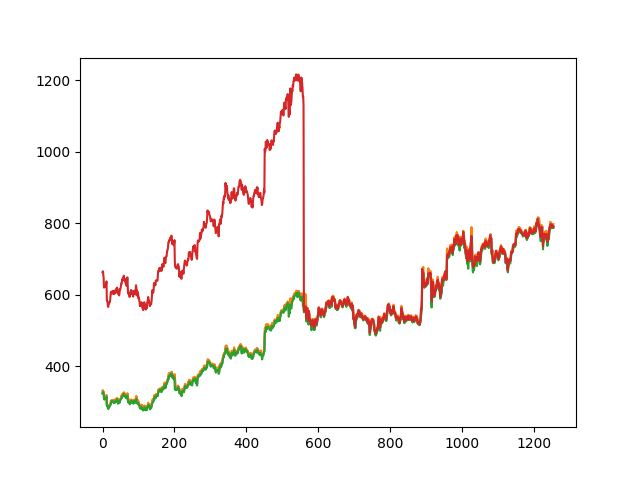
\includegraphics[scale=0.5]{close_no_fix.png}
   \caption{Prices with no close fix }
   \end{figure}
 \end{center}
 \squeezeup
To address this a function was written that divides the close price by two if the 
close price is higher than the High field for that day. At no point should the 
close price be higher than the high price therefore when this condition is met it 
is clear there was a data recording error. Plotting the data after this 
fix can be seen in the below plot.

\begin{center}
   \begin{figure}[H]
   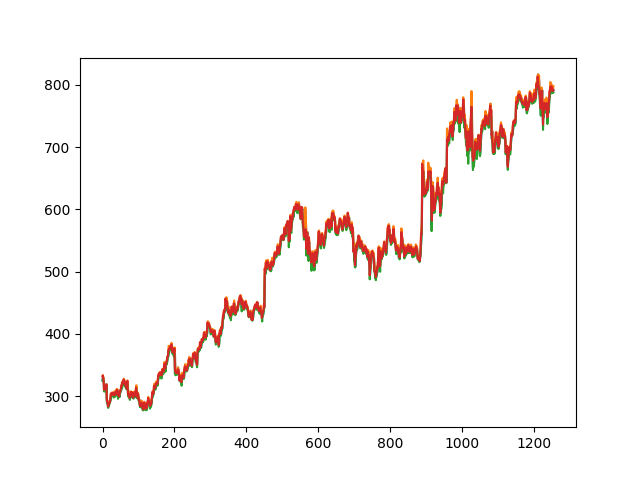
\includegraphics[scale=0.5]{close_fix.png}
   \caption{Prices with close fix }
   \end{figure}
 \end{center}
 \squeezeup

Some data cleaning was also done on the Close field with some of the entries being 
recorded in a string format with quotation marks. Some of the entries also contained 
commas to split the price up. These quotes and commas were removed from the applicable 
entries resulting in a valid numeric entry.

The dataset provided contained two files, a training set and a testing set. The testing 
set contains issues as the dataset does not contain entries for every sequential day.
This causes issues when trying to predict the next day given the previous $n$ days. 
To address this the testing data was largely disregarded and the testing set was 
split up into a standalone training and testing set. The training process is completed 
on the first seventy percent of the data with the remainder being used as the testing set.
Investigating any model performance impacts caused by the split size will be expanded on 
in the future work section. 
\subsection{Metrics}
The metrics used to measeure the performance of the models given the various parameter 
values are RMSE and MAPE. RMSE is defined as
\begin{equation}
   RMSE = \sqrt{\dfrac{\sum_{i=1}^{n}(Y_i - \hat{Y}_i)^2}{n}}
\end{equation}
where $n$ is the number of data points $Y_i$is the observed values and $\hat{Y}_{i}$
is the predicted values. MAPE is defined as
\begin{equation}
   MAPE = \dfrac{1}{n}\sum_{i=1}^{n}\left\lvert\dfrac{A_t-F_t}{A_t}\right\rvert 
\end{equation}
which calculates the percentage difference between the predicted values and the actual 
values.

\subsection{Learning Rate}
The learning rate controls the rate at which the parameters in the network are updated.
A higher learning rate can lead to a quicker training process however it can result 
in overshooting the optimal values. A lower learning rate can cause the model to 
converge slower and also get stuck at local minima. This causes the model not to reach 
its optimal state. To investigate the learning rates a range of values will be tested 
on the models. These values are 0.1,0.01,0.001 and 0.0001.
\subsection{Epochs}
To identify an appropriate epoch value for the training process of each model the loss 
value at each epoch will be calculated and plotted. The loss metric is the difference 
between the models prediction at a given time and the actual value. For the loss, this 
investigation used the Mean Square Error Loss which is defined as
\begin{equation}
   MSE = \dfrac{1}{n}\sum_{i=1}^{n}(Y_i - \hat{Y}_i)^2
\end{equation}
where $n$ is the number of data points $Y_i$is the observed values and $\hat{Y}_{i}$
is the predicted values.

An value will be chosen when the loss stabilises and doesnt noticably improve. To 
account for the rapid improvement during the first set of epoch values tested, the plotted 
will ignore the first twenty epoch values loss values. Without this the scale of the plot
becomes difficult to interperet.

\subsection{Hidden State Size}
The hidden state size is used to define the number of parameters that are calculated 
in each node. Values of 16, 32, 64 and 128 will be tested and their metric results 
calculated.
\subsection{PyTorch}
Although it is possible to build these RNN models from scratch,
open source tools have allowed for rapid development and
implementation of these models. Pytorch is one of these
tools which is available in the Python programming language. Pytorch enables rapid 
prototyping of different models through its publishing of base implementations on a
large number of common machine learning models. For
the models investigated in this report, a base Pytorch implementation was available 
for each of them. Pytorch exposes
low level api calls that allow the user to modify the models
which greatly aids in the types of investigation and experimentation that are 
possible. Pytorch can be used for model
training and testing and provides robust functionality for the
end to end process of defining and then using a given machine learning model. 
Pytorch has native support for running this models on GPU's through its CUDA integration.
CUDA is a parallel computing platform and programming
model developed by NVIDIA  that allows developers to
copy data to supported graphics cards and utilise the highly
parallel architecture inherent to GPU's to increase training
time greatly. Since the training process involves large numbers of operations to be done on matrices, this work can be
parallelised effectively for massive performance gains.
\section{Code}
The code used for this report can be found at,
\href{https://github.com/sjg546/dlf_assignment3}{github.com/sjg546/dlf\_assignment3}

\section {Results}
\subsection{Base Performance}
To set a baseline for how modifying the various parameters impact the final performance 
of the models a baseline must be found. The initial model performance will be measured 
with the previous number of days used to calculate the next days performance set to 3.
The batch size set to 32, the hidden layer size set to 64, the number of layers set to 3,
the learning rate set to 0.0001 and the number of training epochs set to 500. 
The RMSE results for the models can be seen below
\begin{center}
   \begin{tabular}{||c c c c c c||} 
    \hline
    Model & Open & High & Low & Close & Total\\ [0.5ex] 
    \hline\hline
    RNN  & 12.415 & 12.427 & 12.443 & 12.458& 12.415\\ 
    \hline
    GRU  & 16.610 & 16.626 & 16.646 & 16.667& 16.610\\ 
    \hline
    LSTM  & 17.595 & 17.609 & 17.628 &  17.651& 17.595\\ 
    \hline
   \end{tabular}
\end{center}
and the MAPE for the models can be seen below
\begin{center}
\begin{tabular}{||c c c c c c||} 
 \hline
 Model & Open & High & Low & Close & Total\\ [0.5ex] 
 \hline\hline
 RNN  & 1.192 & 1.192 & 1.194 & 1.195& 1.192\\ 
 \hline
 GRU  & 1.624 & 1.624 & 1.625 &  1.629& 1.624\\ 
 \hline
 LSTM  & 1.731 & 1.730 & 1.730 & 1.734& 1.731\\ 
 \hline
\end{tabular}
\end{center}
It can be observed that the best performing model in the base state is the RNN with lower 
RMSE and MAPE values for all fields.
\subsection{Epoch Loss Investigation}
Running the models with base parameters of 3 days predicting the next 1 day, a batch size of 
32, hidden size of 64, 3 layers and a learning rate of 0.0001 yields the following 
figures for the models.
\squeezeup
\begin{center}
   \begin{figure}[H]
   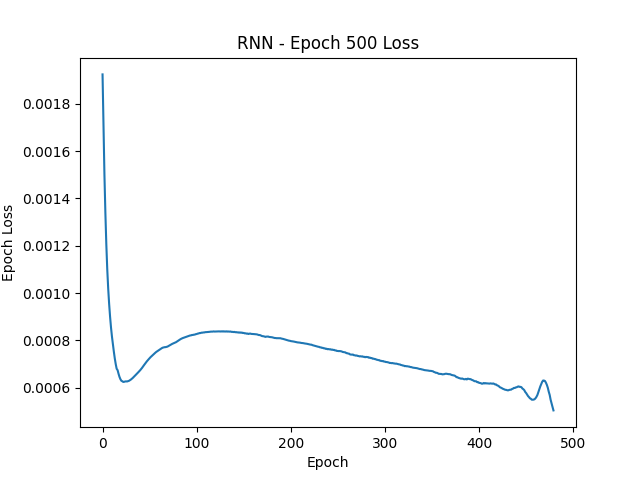
\includegraphics[scale=0.5]{RNN-Epoch500_loss.png}
   \caption{Base RNN Epoch Loss Plot }
   \end{figure}
 \end{center}
 \squeezeup

It can be observed that the loss rapidly decreases until an epoch of approximately 40, then 
spikes before reducing consistently to approximately 450. The GRU model yields a curve shown
below.

\begin{center}
   \begin{figure}[H]
   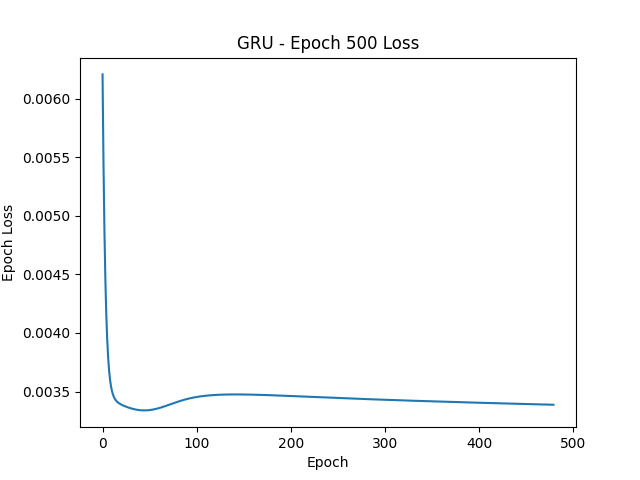
\includegraphics[scale=0.5]{GRU-Epoch500_loss.png}
   \caption{GRU Epoch Loss Plot }
   \end{figure}
 \end{center}
 \squeezeup

Similarly the GRU models loss rapidly decreases until an epoc value of approximately 60
before increasing slightly. It can also be observed that the GRU loss is significantly 
higher than the RNN. Investigating the impact of increasing the epoch greatly to 3000 yields 
a loss plot of.
\begin{center}
   \begin{figure}[H]
   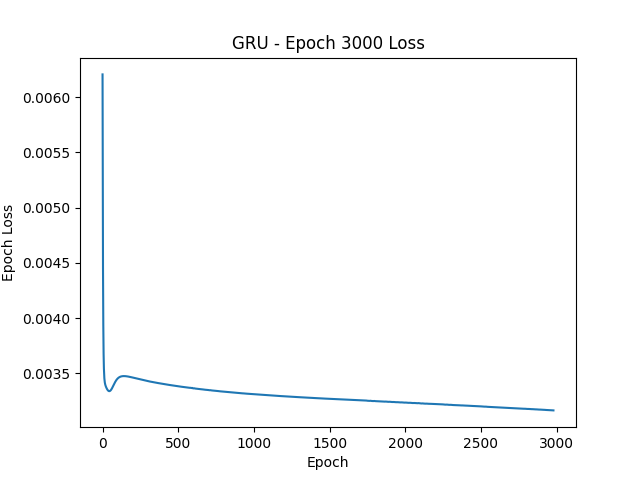
\includegraphics[scale=0.5]{GRU-Epoch3000_loss.png}
   \caption{GRU Epoch 3000 Loss Plot}
   \end{figure}
 \end{center}
This plot shows that although the loss does continue to reduce as the epoch number increases 
the gains are marginal with the loss only reducing to ~0.0031 with 3000 epochs. Balancing 
the time required to train the model with this and the marginal improvement in the lowered 
loss an epoch value of 500 was chosen.The results for the LSTM 
were finally calculated and plotted below. 
\begin{center}
   \begin{figure}[H]
   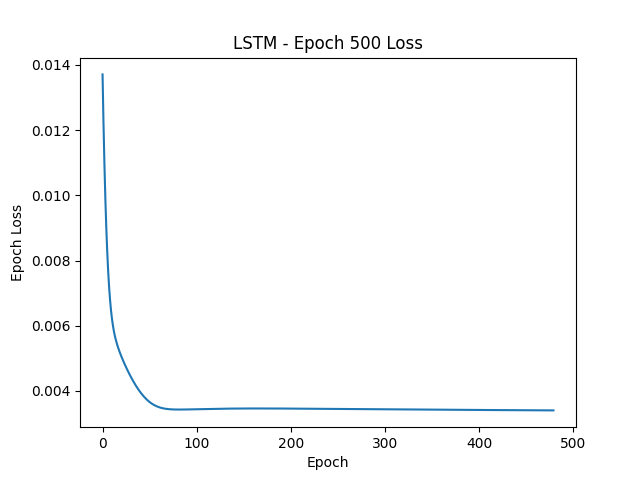
\includegraphics[scale=0.5]{LSTM-Epoch500_loss.png}
   \caption{LSTM Epoch Loss Plot }
   \end{figure}
 \end{center}
 \squeezeup

The LSTM results are similar to the GRU results however the loss doesnt appear to spike as 
drastically after initially reaching a local minima. Again, the loss values are significantly 
higher than the base RNN implementation.
\subsection{Learning Rate Investigation}
The impact of the learning rate on the models performace will be investigated by running the 
GRU model with various values. The GRU model strikes a balance between the complexities of 
the base RNN model and the LSTM. The results for the RMSE metric can be seen below
\begin{center}
   \hspace*{-0.8cm}
   \begin{tabular}{||c c c c c c||} 
    \hline
    LR & Open & High & Low & Close & Total\\ [0.5ex] 
    \hline\hline
    0.1  & 124.768& 123.893& 123.027& 122.194& 124.768\\ 
    \hline
    0.01  & 23.406& 23.418& 23.435& 23.462& 23.406 \\
    \hline
    0.001  & 15.044& 15.050& 15.065& 15.084& 15.044 \\
    \hline
    0.0001  & 16.611& 16.626& 16.646& 16.668& 16.611 \\
    \hline
    0.00001 & 16.228& 16.242& 16.261& 16.282& 16.228 \\
    \hline
   \end{tabular}
\end{center}
and the MAPE results are   
\begin{center}
   \begin{tabular}{||c c c c c c||} 
    \hline
    LR & Open & High & Low & Close & Total\\ [0.5ex] 
    \hline\hline
    0.1  & 16.219& 16.102& 15.987& 15.876& 16.219\\ 
    \hline
    0.01   & 2.622& 2.619& 2.618& 2.621& 2.622 \\
    \hline
    0.001  & 1.570& 1.568& 1.568& 1.571& 1.570 \\
    \hline
    0.0001  & 1.624& 1.624& 1.626& 1.629& 1.624 \\
    \hline
    0.00001  & 1.560& 1.560& 1.561& 1.564& 1.560 \\    
    \hline
   \end{tabular}
\end{center}
It can be observed that there is minimal improvement for learning rates smaller than 0.001.
to avoid a slow training process whilst balancing model performance a learning rate of 
0.001 is appropriate.
\subsection{Hidden Layer Size Investigation}
Similar to the learning rate investigation the GRU model will be used to investigate the 
impact modifying the hidden layer size has on performance. The results for the RMSE metric can be seen below
\begin{center}
   \begin{tabular}{||c c c c c c||} 
    \hline
    Size & Open & High & Low & Close & Total\\ [0.5ex] 
    \hline\hline
    16  & 16.569& 16.578& 16.592& 16.613& 16.569 \\
    \hline
    32  & 15.366& 15.377& 15.394& 15.414& 15.366 \\
    \hline
    64  & 15.044& 15.050& 15.065& 15.084& 15.044 \\
    \hline
    128  & 15.511& 15.520& 15.535& 15.556& 15.511 \\
    \hline
   \end{tabular}
\end{center}
and the MAPE results are   
\begin{center}
   \begin{tabular}{||c c c c c c||} 
    \hline
    Size & Open & High & Low & Close & Total\\ [0.5ex] 
    \hline\hline
    16   & 1.730& 1.728& 1.728& 1.731& 1.730 \\
    \hline
    32  & 1.596& 1.595& 1.596& 1.599& 1.596 \\
    \hline
    64 & 1.570& 1.568& 1.568& 1.571& 1.570 \\
    \hline
    128  & 1.621& 1.619& 1.620& 1.623& 1.621 \\
    \hline
   \end{tabular}
\end{center}
From the above it can be seen that the best performing hidden layer size is 64.
\subsection{Final Results}
After running the GRU model with all the found parameters from the investigations 
the final total RMSE and MAPE was found to be 15.044 and 1.570 respectively. This 
is a reduction in RMSE of 1.55 and MAPE of approximately 0.06. The plotted predictions 
for the close price of the stock against the actual values can be seen below.
\begin{center}
   \begin{figure}[H]
   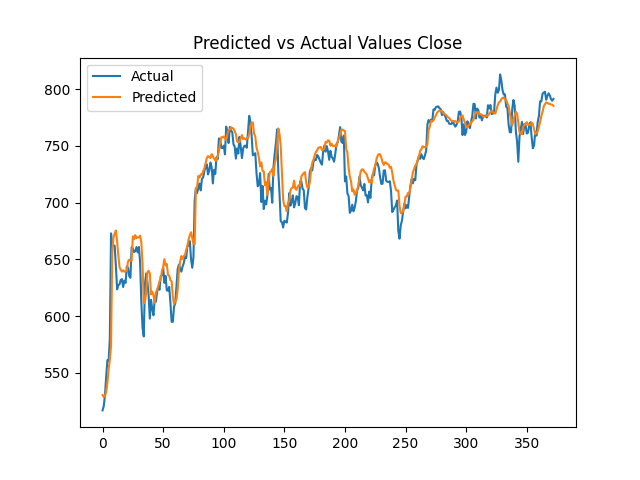
\includegraphics[scale=0.5]{GRU_Close.png}
   \caption{Predicted vs Actuals GRU Model - Close Price }
   \end{figure}
 \end{center}
 \squeezeup
From this plot it can be observed that the model does an excellent job of capturing the 
trajectory and prices of the stock over time.
\section{Discussion}
From the results it can be observed that the best performing model is the base RNN. For both 
training loss and performance metrics the RNN outperformed the GRU and the LSTM. It was 
expected that the long term memory capabilities of the GRU and LSTM should increase performance.
This was not observed, potentially because of the smaller testing set that was used.
This long term memory capability should be able to capture seasonal trends in the stock 
price fluctuations. By splitting the dataset into 70\% training and 30\% testing the 
data available to train the model on these seasonal cycles are limited. This was also observed
with the GRU model. This limited training data and inconsistent provided test data 
greatly limited the performance of the models. Expanding the data used for training and 
testing will be expanded on in the future work section of this report.
The base RNN performed extremely well on the data provided. It greatly outperformed the 
GRU and LSTM. The base RNN's quick training time and performance makes it the clear selection 
for this problem space with the given parameters. Where it may struggle is during future 
work where different stocks are provided to the model. For stocks that are much succeptible 
to seasonal swings the RNN will struggle to accurately capture those. 
Modifying the parameters used when training the model tangibly improved the models performance.
When using the found parameters for the GRU model, the overall RMSE of the models predictions 
improved by approximately 1.55 or a ten percent improvement. This was achieved by some 
rudimentary parameter sweeping. Further improvements may be able to be achieved by using 
more comprehensive parameter searching techniques such as gradient based optimisation.
By finding the optimal values for the models such that the training loss is minimised 
and the predictions are as accurate as possible, the maximum performance of the models  
given their current implementations can be found.

\section{Future Work}
To expand the scope of this project there are a few natural follow on pieces of work that 
have been identified. The first is to investigate the impact of the specific test train 
split used on the dataset. Determining if better performance can be achieved by reducing
the amount of test data is used will form the basis of this. Following on from that,
using the system as built and determining its performance on a broad range of different 
stocks. This investigation has been solely focussed on google stock prices, determining 
if the performance of the models generalises to other stocks is important. This will 
potentially allow for more data to be obtained thus allowing the other models with longer 
memories to perform better. 
The models have been setup to only predict the next days results given the subsequent $n$
days performance. Extending this to predict a set of future days will increase the models 
flexibility and usability. This will involve modifying the various models forward functions 
to support this. A possible extension that can be made to the LSTM model is to add attention 
to it. Attention allows the model to focus on important parts of the input sequence when 
making predictions. Attention works by calculating a score for each hidden state which 
represents its importance to the current prediction. This attention module should allow 
the model to more accurately predict future stock prices.
Finally an adaption of this model will be investigeted to predict whether or not the next 
days stock price will be up or down. Converting this into a binary regression problem 
could provide value to users.

%-------------------------------------------------------------------------
\small
\bibliographystyle{ieee_fullname}
\bibliography{egbib}

\end{document}
